\newpage
\section*{Referencias}
\textbf{Básico: }
\begin{itemize}
	\item \textit{Problema 1.} Problema 1 Final UIS 2018 Nivel Avanzado Primaria. 
	\item \textit{Problema 2.} Problema 2 Final UIS 2018 Nivel Avanzado Primaria. 
	\item \textit{Problema 3.} Problema 8 Selectiva UIS 2012 Nivel Medio Primaria.
	\item \textit{Problema 4.} Problema 9 Selectiva UIS 2012 Nivel Medio Primaria.
	\item \textit{Problema 5.} Creado.
\end{itemize}

\textbf{Avanzado: }
\begin{itemize}
	\item \textit{Problema 1.} Problema 8 Selectiva UIS 2019 Nivel Avanzado
	\item	\textit{Problema 2.} Problema 2 Selectiva UIS 2018 Nivel Avanzado
	\item	\textit{Problema 3.} 4.55 de \textit{Introduction to Number Thoery (AOPS)}
	\item	\textit{Problema 4.} Problema 2 Geometría N.2 A.4 de POTI (	Programa Olímpico de Treinamento)
	\item	\textit{Problema 5.} 2.31 de David Patrick. \textit{Introduction to Counting and Probability}. Aops, 2005.
\end{itemize}

%------------------------------------------------------------------------------------------------------------   
%----------------------------------                        BASICO                       ---------------------------------- 
%------------------------------------------------------------------------------------------------------------ 

\newpage
\section{Nivel Básico}\label{basico:2020_15_agosto}

\begin{center}
	\fbox{\fbox{\parbox{6in}{\centering
				\textbf{Tiempo mínimo: } 2 horas y 30 minutos.\\
				\textbf{Tiempo máximo: } 4 horas.\\	
				\textbf{Procedimientos: }Cada problema debe estar resuelto por escrito, en forma detallada, todos los pasos seguidos para su resolución deben estar bien explicados. Se le brindarán unas hojas grapadas, en la \textit{parte de enfrente} de cada hoja debe estar la solución de los problemas, la \textit{parte posterior} no se leerá pero las operaciones y cálculos deben hacerlos allí. \\
				\textbf{Puntaje: }Cada problema vale 50 puntos, son 5, para un total de 250 puntos.
				}}}
\end{center}

\begin{enumerate}
	\item \textbf{(50 puntos)}. 
				\begin{figure}[H]
					\centering
					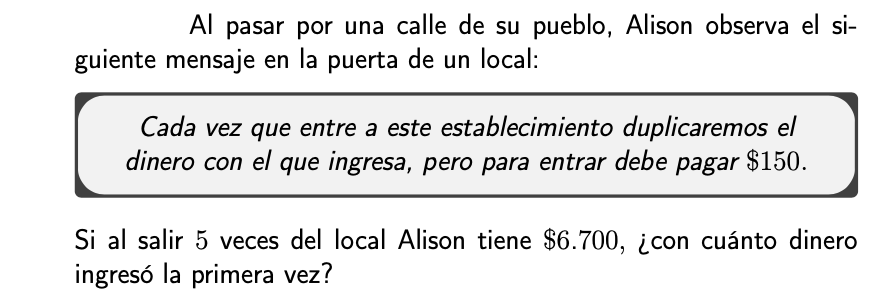
\includegraphics[width=0.95\linewidth]{2020_08_15/imgs/basicoproblema1}
					%\caption{}
					\label{fig:basicoproblema1}
				\end{figure}
			
	\item \textbf{(50 puntos)}. 
				\begin{figure}[H]
					\centering
					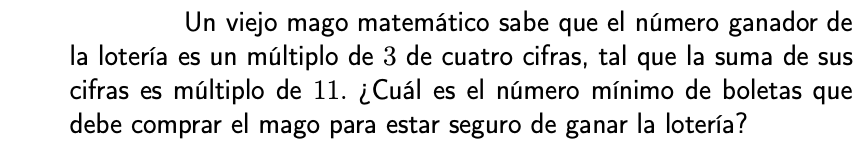
\includegraphics[width=0.95\linewidth]{2020_08_15/imgs/basicoproblema2}
					%\caption{}
					\label{fig:basicoproblema2}
				\end{figure}
	
		\item \textbf{(50 puntos)}. 
				\begin{figure}[H]
					\centering
					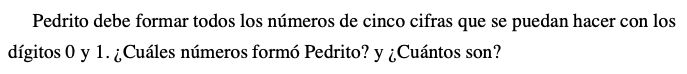
\includegraphics[width=0.95\linewidth]{2020_08_15/imgs/p8basico}
					%\caption{}
					\label{fig:basicoproblema3}
				\end{figure}

	\item \textbf{(50 puntos)}. 
			\begin{figure}[H]
				\centering
				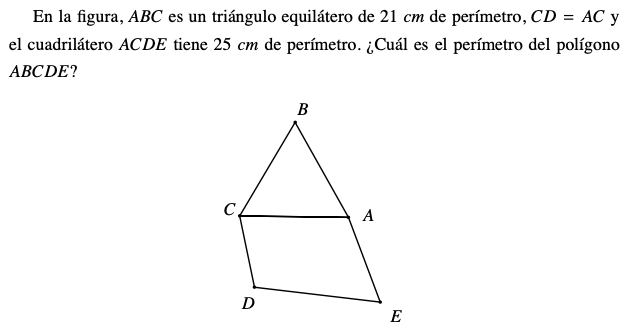
\includegraphics[width=0.95\linewidth]{2020_08_15/imgs/p9basico}
				%\caption{}
				\label{fig:basicoproblema4}
			\end{figure}
		
	\item \textbf{(50 puntos)}. Calcular el resultado de la siguiente operación:
	\[
	\frac{100-101+102-103+104-105+106-\cdots +198-199+200}{50}
	\]
\end{enumerate}



%------------------------------------------------------------------------------------------------------------   
%----------------------------------                        AVANZADO                       ---------------------------------- 
%------------------------------------------------------------------------------------------------------------ 

\newpage
\section{Nivel Avanzado}\label{avanzado:2020_15_agosto}

\begin{center}
	\fbox{\fbox{\parbox{6in}{\centering
				\textbf{Tiempo mínimo: } 2 horas y 30 minutos.\\
				\textbf{Tiempo máximo: } 4 horas.\\		
				\textbf{Procedimientos: }Cada problema debe estar resuelto por escrito, en forma detallada, todos los pasos seguidos para su resolución deben estar bien explicados. Se le brindarán unas hojas grapadas, en la \textit{parte de enfrente} de cada hoja debe estar la solución de los problemas, la \textit{parte posterior} no se leerá pero las operaciones y cálculos deben hacerlos allí. \\
				\textbf{Puntaje: }Cada problema vale 50 puntos, son 5, para un total de 250 puntos.
	}}}
\end{center}


\begin{enumerate}
		\item \textbf{(50 puntos)}. 
		\begin{figure}[H]
			\centering
			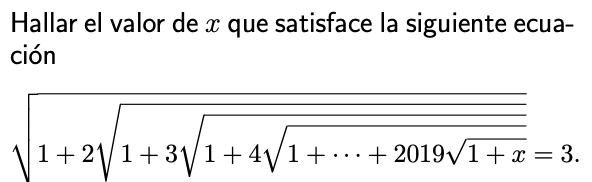
\includegraphics[width=0.6\linewidth]{2020_08_15/imgs/p8selectivavanzado2019}
			%\caption{}
			\label{fig:p8selectivavanzado2019}
		\end{figure}

\item \textbf{(50 puntos)}. 
		\begin{figure}[H]
			\centering
			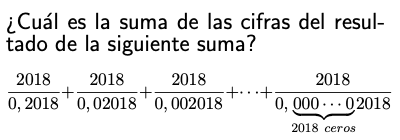
\includegraphics[width=0.6\linewidth]{2020_08_15/imgs/p2selectivaavanzado2018}
			%\caption{}
			\label{fig:p2selectivaavanzado2018}
\end{figure}

\item \textbf{(50 puntos)}.  Cualquier producto entre dos de los números 30,72 y $N$ es divisible por el tercero. Cuál es el valor mas pequeño posibile que puede tener $N$?

\item \textbf{(50 puntos)}. En un $\triangle ABC$, $AB=4cm,BC=5cm$ y $AC=6cm$. Calcular la medida de los lados un triángulo semejante a $ABC$ que tenga perímetro $20cm$.

\item \label{problema:15agNOON} \textbf{(50 puntos)}. De cuántas formas usted puede deletrar la palabra NOON a partir de la tabla que se muestra debajo? Para deletrear usted puede empezar con cualquier letra, luego en cada paso usted se puede mover arriba, abajo, a la derecha, a la izquierda o en diagonal hasta que termine de deletrar la palabra. Usted no puede pasar por la misma casilla dos veces. 

\begin{table}[H]
	\centering
	\begin{tabular}{|l|l|l|l|}
		\hline
		N & N & N & N \\ \hline
		N & O & O & N \\ \hline
		N & O & O & N \\ \hline
		N & N & N & N \\ \hline
	\end{tabular}
	%\caption{Problema \ref{problema:15agNOON}.}
	%\label{tabla_NOON}
\end{table}	
\end{enumerate}